\section{Analysis}

For better understanding the ICL training strategy, 
we combined it with the traditional CL and did comprehensive ablation studies. All of the experiments in this section are done on the SAMSum dataset, which is representative due to the medium output length.

\subsection{Combinations with the Traditional CL}

We design $4$ different strategies n ranking samples in the training set for dialogue summarization empirically as follows:
\begin{itemize}
	\item \textbf{Input length (InLen)} refers to the number of tokens in the input dialogue. The longer a dialogue is, the more complex a sample is.
	\item \textbf{Output length (OutLen)} is the number of tokens in a reference summary, which is also proportional to the difficulty of a sample.
	\item \textbf{Compression ratio (CompR)} equals the output length divided by the input length. We generally agree that more compressed training pairs are harder for models to lean from.
	\item \textbf{Abstractiveness (Abstr)} represents the percentage of novel words appearing in the reference summary which are not in the dialogue. We use Rouge-2 recall as the abstractiveness score, which is inversely proportional to the difficulty level.
\end{itemize}

The results based on the ordered training set according to these intuitive CL strategies are shown in Table~\ref{tab:traditional}. It shows that only InLen improves the vanilla model, but it still lags behind our results in Table~\ref{tab:end2endds}. Other strategies failed mainly due to the low data quality at the beginning or the end of training. 
Taking Abstr as an example, samples with the highest 
Rouge-2 recall are gathered at the beginning where 
their inputs and outputs are almost the same. 
This leads to a bad initialization for models learning 
the summarization ability. Besides, some strategies 
are incompatible, such as OutLen and CompR. Samples with the shortest output length are always too compressed. Therefore, it's hard to develop a comprehensive score for better ranking. It should be also notice that most of these strategies are developed based on the target of dialogue summarization task, which are not suitable for generalization. In a word, it's hard to develop a 
comprehensive strategy for a single task or a unified strategy for different NLG tasks based on the traditional CL. 

Our ICL strategy can be simply combined with these CL strategies by training with the ordered training set instead of the random sampling. The ICL not only outperforms these CL baselines, but also improves them when combined together. 

\label{sec:tracl}
\begin{table}[t]
	\scriptsize
	\centering
	\begin{tabular}{lccccc}
		\hline
		{Method} & {R1} & {R2} & {RL} & {Met} & {BertS} \\
		\hline
		InLen & 52.19 & \textbf{27.73} & \textbf{43.50} & 25.57 & 71.73\\
		InLen+ & \textbf{52.56} & 27.60 & 43.43 & \textbf{25.77} & \textbf{71.92}\\
		\hline
		OutLen & 41.38 & 20.88 & 31.77 & \textbf{27.95} & 67.21\\
		OutLen+ &\textbf{43.96} & \textbf{22.14} & \textbf{33.05} & 26.39 & \textbf{67.64} \\
		\hline
		CompR & 39.68 & 19.28 & 34.73 & 14.41 & 65.96 \\
		CompR+ & \textbf{41.59} & \textbf{20.78} & \textbf{26.62} & \textbf{15.22} & \textbf{67.19}\\
		\hline
		Abstr & \textbf{44.61} & 20.10 & 36.93 & \textbf{17.34} & 68.29 \\
		Abstr+ & 44.41 & \textbf{20.64} & \textbf{37.29} & 17.25 & \textbf{68.33} \\
		\hline
	\end{tabular}
	\caption{Ablations on propotional ICL strategies}
	\label{tab:traditional}
\end{table}

%\subsection{Performance on Variable Lengths}

%\begin{table}
%	\small
%	\centering
%	\begin{tabular}{lcccccc}
%	\hline
%	Dataset &  Avg & Std & \#1 & \#2 & \#3 & \#4 \\
%	\hline
%	DREAM & 5.59 & 2.61 & 483 & 653 & 468 & 483 \\
%	\hline
%	SAMSum & 24.99 & 13.06 & 227 & 260 & 170 & 162 \\	
%	\hline
%	\multirow{2}{*}{Shakespeare} & 12.24 & 9.27 & 423 & 288 & 290 & 461 \\
%	& 11.02 & 7.10 & 423 & 328 & 264 & 447 \\
%	\hline
%	SQuAD1.1 & 13.09 & 4.27 & 2330 & 4755 & 3041 & 1751 \\
%	\hline
%	CNNDM & \\
%	\hline
%	\end{tabular}
%	\caption{Statistics on variable output length. Avg and Std refer to the average and the standard deviation of the output length. \#1 to \#4 represent the number of samples belonging to different test buckets divided by the output length in ascending order.
%	Shakespeare contains two rows as its output can be in both styles.}
%	\label{tab:ablength}
%\end{table}

%\begin{figure*}[th]
%	\centering

%		\begin{minipage}[t]{0.5\linewidth}
%			\centering
%				\subfloat[Dialogue Summarization]{
%			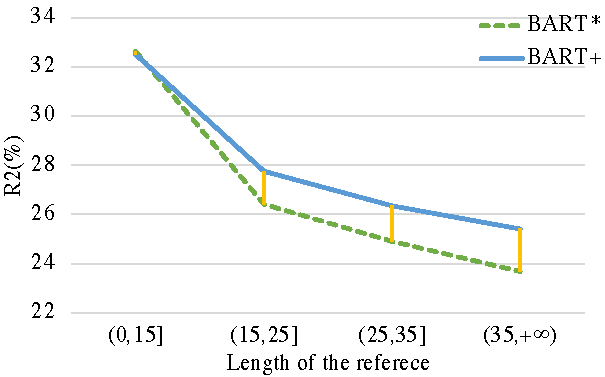
\includegraphics[scale=0.65]{length-ds.pdf}
			%\caption{fig1}
%				}%
%		\end{minipage}%
%		\begin{minipage}[t]{0.5\linewidth}
%			\centering
%				\subfloat[Reading Comprehension]{
%			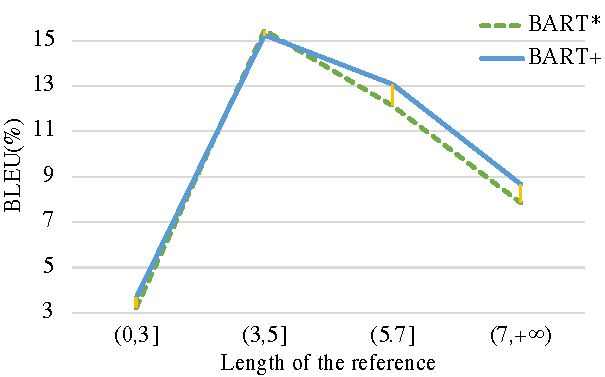
\includegraphics[scale=0.65]{length-rc.pdf}
			%\caption{fig2}
%				}%
%		\end{minipage}%
	
%		\begin{minipage}[t]{0.5\linewidth}
%			\centering
%			\subfloat[Style Transfer]{
%				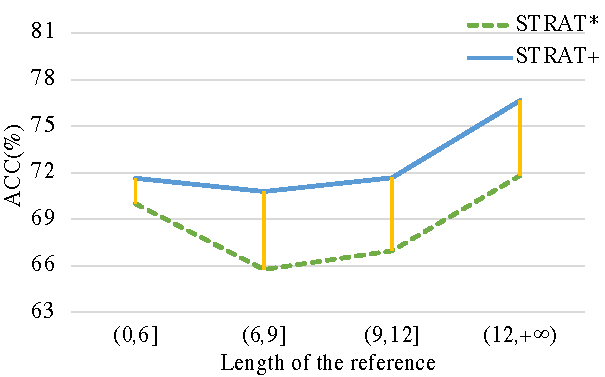
\includegraphics[scale=0.65]{length-st.pdf}
				%\caption{fig2}
%			}%
%		\end{minipage}%
%		\begin{minipage}[t]{0.5\linewidth}
%			\centering
%			\subfloat[Question Generation]{
%				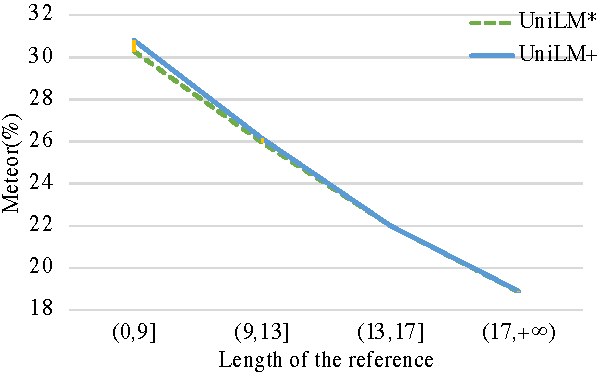
\includegraphics[scale=0.65]{length-qg.pdf}
				%\caption{fig2}
%			}%
%		\end{minipage}
%	\centering
%	\caption{Comparisons on variable lengths. \KZ{The label should read
%Length of the ``reference'' text.}}
%	\label{fig:ablength}
%\end{figure*}


\subsection{Ablations on the Training Strategy}

%1. strategy: increase; decrease; random
To understand the design of decreasing the prefix for ICL, we introduce the ablation on training strategies as follows:
\begin{itemize}
	\item \textbf{Decrease} refers to the Algorithm~\ref{alg:picl}. Taking $p_{start}=0.6$ and $s=0.3$ as an example, the prefix percentage $p$ varies as $0.6\rightarrow 0.3\rightarrow 0.0$ during training.
	\item \textbf{Increase} means that we gradually increase the length of prefix by increase $p$ following $0.0\rightarrow0.3\rightarrow0.6$.
	\item \textbf{Random} is that we randomly pick $p$ from the set $\{0.0, 0.3, 0.6\}$ in this example.
\end{itemize}

The results are shown in Table~\ref{tab:ablstrategy}. Decrease significantly outperforms other ablations, showing that this strategy works by means of learning from easy to hard, instead of the implicit ``data augmentation'' which calculates different losses given the same sample during training.

\begin{table}[th]
	\scriptsize
	\centering
	\begin{tabular}{cccccc}
		\hline
		{Stra.} & {R1} & {R2} & {RL} & {Met} & {BertS} \\
		\hline
		Decrease &\textbf{53.07} & \textbf{28.23} & \textbf{43.83} & \textbf{26.12} & \textbf{72.17}\\
		Increase & 51.89 & 27.33 & 42.80 & 25.24 & 71.40 \\
		Random & 51.58 & 27.17 & 43.03 & 23.91 & 71.24 \\
		\hline
	\end{tabular}
	\caption{Ablations on ICL strategies. The starting point and the stride are 0.6 and 0.3 respectively.}
	\label{tab:ablstrategy}
\end{table}


\subsection{Ablations on the Starting Point and the Stride}

To better understand how the ICL manipulates the difficulty of samples during the training process, we further did experiments on different settings of two newly-introduced hyper-parameters $p_{start}$ and $s$. The results are shown in Table~\ref{tab:ablstart}.

We can see that the performance drops with either a too large or too small $p_{start}$. The former one starts training with only predicting the last 1 or 2 tokens according to the average length of reference output shown in Table~\ref{tab:taskdata}. Most of times, they are punctuation marks which do not carry any important semantic information, leading to a bad warm-up. The latter one requires the model to predict more than half of the output, which are too difficult as a beginning learning target.
All of the results still outperforms the original baseline.

The trend is the same for using different stride values. The performance even drops with the strides equaling 0.1 or 0.6. 
The former one leads to too little changes, which not only excessively prolongs the required training time but also leads to server outfitting on the training set. The latter one greatly enlarges the gap between training targets which degrades to 0.0 directly. It also harms the performances.

In a word, the training should start with a medium difficulty training objective and the gap between training objectives should be too large. Both parameters are closely related to the output length of different tasks. Based on these ablations, we suggest using ($p_{start}=0.6$, $s=0.3$) for NLG tasks with multi-sentence outputs, and ($p_{start}=0.5$, $s=0.5$) for NLG tasks with sing-sentence outputs. All of our experiments above are done based on this guideline. More insights on the relation between the average output length and parameter settings are expected as future work.

%2. hyper-parameters of starting point: 0.6,0.7,0.8,0.9,  0.3,0.4,0.5

\begin{table}[t]
	\scriptsize
	\centering
	\begin{tabular}{ccccccc}
		\hline
		{Start} & {Stride}& {R1} & {R2} & {RL} & {Met} & {BertS} \\
		\hline
		0.9 &\multirow{7}{*}{0.3}& 52.97 & 27.86 & {43.72} & \textbf{26.23} & 71.89 \\
		0.8 & &52.54 & 27.54 & 43.44 & 26.08 & 71.92 \\
		0.7 & &51.44 & 26.73 & 42.74 & 25.26 & 71.32 \\
		0.6 & &\textbf{53.07} & \textbf{28.23} & \textbf{43.83} & 26.12 & \textbf{72.17}\\
		0.5 & &52.37 & 27.78 & 43.54 & 25.31 & 71.74 \\
		0.4 & &52.14 & 27.68 & 43.20 & 25.09 & 71.52 \\
		0.3 & &51.46 & 27.30 & 42.74 & 24.37 & 71.15\\
		\hline
		\multirow{6}{*}{0.6}&0.1  & 50.75 & 26.04 & 41.86 & 24.06 & 70.81\\
		&0.2 & 52.46 & 28.02 & 43.63 & 25.21 & 71.79\\
		&0.3 & \textbf{53.07} & \textbf{28.23} & \textbf{43.83} & \textbf{26.12} & \textbf{72.17} \\
		&0.4 & 51.90 & 27.73 & 43.09 & 25.11 & 71.53\\
		&0.5 & 51.84 & 27.68 & 43.15 & 24.99 &71.73\\
		&0.6 & 50.86 & 26.68 & 42.32 & 23.55 &70.76\\
		\hline
		w/o & w/o &51.88 & 27.30 & 42.77 & 24.75 & 71.38 \\
		\hline
	\end{tabular}
	\caption{Ablations on the starting point of propotional ICL with the stride equaling 0.3 and ablations on the stride of propotional ICL with the starting point equaling 0.6. The last line with ``w/o'' representing the BART baseline without using the ICL strategy is listed for comparison.}
	\label{tab:ablstart}
\end{table}

\begin{table}[th!]
	\small
	\centering
	\begin{subtable}{\linewidth}
		\scriptsize
		\centering
		\begin{tabular}{p{1cm}p{5.8cm}}
			\toprule[1pt]
			{Dialogue} & \makecell[l]{M: Hi, is that Sara?\\
				W: Speaking. \\
				M: This is Tom. Sorry to bother \textbf{you} \textbf{at supper time}.\\
				W: Not at all.\\
				M: My little girl Maria has a high fever. We're taking her to \\\quad hospital in a short time.\\
				W: I'm sorry to hear that. Is there anything I can do for you? \\
				M: Do you mind taking care of my son Ken? We can't take\\\quad him along. \\
				W: OK. Can I bring him to my house?\\
				M: Thank you. But he hasn't finished his dinner yet.\\
				W: No problem. He can {have dinner with us}, and then, my \\\quad son will play games with him.\\
				M: I really appreciate your help.
			} \\
			\hline
			Question & What is the woman doing at the moment?\\
			\hline
			Reference & Having supper. \\
			\hline
			w/o CL & She is \textbf{\textit{taking care of her daughter}}.\\
			\hline
			TCL & She is \textbf{\textit{talking to someone}}. \\
			\hline
			ICL & She is having supper. \\
			
			
			
			\midrule[1pt]	
			{Dialogue} & \makecell[l]{F: When shall\ start, at four or at five? \\
				M: How about \textbf{half past four}?}\\
			\hline
			{Question} & When does the man want to start?\\
			\hline
			{w/o CL} & At \textbf{\textit{4:45}}. \\
			\hline
			{TCL} & At \textbf{\textit{4:45}}. \\
			\hline
			ICL & At \textbf{\textit{4:00}}. \\
			\bottomrule[1pt]
		\end{tabular}
		\caption{Reading comprehension}
		\label{tab:caserc}
	\end{subtable}
	\\[5pt]
	\begin{subtable}{\linewidth}
		\scriptsize
		\centering
		\begin{tabular}{p{1cm}p{5.8cm}}
			\toprule[1pt]
			{Dialogue} & \makecell[l]{Blake: where r u men? \\
				George: comin'!\\
				Blake: good} \\
			\hline	
			{Reference} & George is coming to a meeting with Blake.\\
			\hline
			
			w/o CL & George and Blake are going to meet.\\
			\hline
			TCL & \textbf{\textit{GeorgeGeorge}} and his friends are coming to Blake.\\
			\hline
			ICL & George and Blake are meeting. \\
			\bottomrule[1pt]
		\end{tabular}
		\caption{Dialogue summarization}
		\label{tab:caseds}
	\end{subtable}
	\\[5pt]
	\begin{subtable}{\linewidth}
		\scriptsize
		\centering
		\begin{tabular}{p{1cm}p{5.8cm}}
			\toprule[1pt]
			{Modern} & \makecell[l]{Were you talking about Juliet ?} \\
			\hline	
			{Original} & Spakest \textbf{thou} of Juliet ?\\
			\hline	
			w/o CL &Did you hear of Juliet ?\\
			\hline
			TCL & Did you hear of Juliet ?\\
			\hline
			ICL & \textbf{Didst thou} hear of Juliet ?\\
			\midrule[1pt]
			{Modern} & \makecell[l]{We have a little dessert coming up .} \\
			\hline	
			{Original} & We have \textbf{a trifling foolish banquet} towards. Is it e'en so ?\\
			\hline
			w/o CL &Let's have some \textbf{{sweets}} .\\
			\hline
			TCL & We'll have some \textbf{{dessert}} .\\
			\hline
			ICL & Let's have some \textbf{{dainties}} .\\
			\bottomrule[1pt]
		\end{tabular}
		\caption{Style Transfer}
		\label{tab:casest}
	\end{subtable}
		\\[5pt]
	\begin{subtable}{\linewidth}
		\scriptsize
		\centering
		\begin{tabular}{p{1cm}p{5.8cm}}
			\toprule[1pt]
			{Document} & {Despite his success as a producer, West's true aspiration was to be a rapper. Though he had developed his rapping long before he began producing, it was often a challenge for West to be accepted as a rapper, and he struggled to attain a record deal. Multiple record companies ignored him because he did not portray the gangsta image prominent in mainstream hip hop at the time. \textbf{After a series of meetings with Capitol Records, West was ultimately denied an artist deal.}} \\
			\hline	
			Answer & Capitol Records\\
			\hline
			{Reference} & What label declined to work with Kanye after many meetings?\\
			\hline
			w/o CL & Who was West ' s record label ?\\
			\hline
			TCL & Who was West ' s record label ?\\
			\hline
			ICL & What record company was West denied a record deal ? \\
			\bottomrule[1pt]
		\end{tabular}
		\caption{Question Generation}
		\label{tab:caseqg}
	\end{subtable}
	\caption{Case studies. 
%Due to the space limitation, case studies for question generation and news summarization are in Appendix~\ref{}. 
The \textbf{keywords} are highlighted in bold. And \textbf{\textit{doubtful generations}} are in bold and italic.}
	\label{tab:cases}
\end{table}

 
\subsection{Case Studies}

We show some cases from different tasks in Table~\ref{tab:cases} and analysis as follows.

In the first case of reading comprehension, our model reasons correctly by recognizing ``you'' before ``at supper time'' refers to the women. While the original approach failed on clarifying ``who is taking care of whose daughter''. The answer generated by TCL is also partially reasonable although it's not agree with the reference. The second case shows that the commonsense knowledge, i.e. ``half past four'' is ``4:30'', is lack in all models.

For Dialogue summarization, summaries generated by both the vanilla BART model and our ICL approach both results in good performances on this single sample. Unfortunately, TCL suffers from both lexical problems, including repetition (``GeorgeGeorge'' for ``George'') and missing (``W'' for ``Wendy'' in other cases), caused by their token-level data augmentation design as discussed Section~\ref{sec:intro}. These incorrect augmented samples hurt the language modeling ability.

In contrast, according to the cases in style transfer, our model did better language modeling, reflected by generating more suitable words for transferring to the style of Shakespeare. 
It's the same in the aspect of modeling named entities in language models that ICL succeed to recognize ``Capitol Records'' as a company name instead of a person name shown in the case of question generation.


%3. hyper-parameters of interval: 0.1, 0.2, 0.3, 0.4, 0.5, 0.6

%\begin{table}[th]
%	\small
%	\centering
%	\begin{tabular}{cccccc}
%		\hline
%		{Stride} & {R1} & {R2}& {RL} & {Met} & {BertS} \\
%		\hline
%		0.1  & 50.75 & 26.04 & 41.86 & 24.06 & 70.81\\
%		0.2 & 52.46 & 28.02 & 43.63 & 25.21 & 71.79\\
%		0.3 & \textbf{53.07} & \textbf{28.23} & \textbf{43.83} & \textbf{26.12} & \textbf{72.17} \\
%		0.4 & 51.90 & 27.73 & 43.09 & 25.11 & 71.53\\
%		0.5 & 51.84 & 27.68 & 43.15 & 24.99 &71.73\\
%		0.6 & 50.86 & 26.68 & 42.32 & 23.55 &70.76\\
%		\hline
%		w/o & 51.88 & 27.30 & 42.77 & 24.75 & 71.38 \\
%		\hline
%	\end{tabular}

	
%	\caption{Ablations on the stride of propotional ICL with the starting point equaling 0.6.}
%	\label{tab:ablstride}
%\end{table}

